% chktex-file 44
\section{Results}

\subsection{Comparing ZCNT and CNT}\label{section:comp_dist_res}

\begin{figure}[ht]
    \centering
    \includegraphics[width=0.45\textwidth]{figures/dist_fig_hist.png}
    \caption{Relative error for the pairwise-distances of CNT, CN3, and ZCNT methods on simulated data as described in Section~\ref{section:comp_dist}. This includes errors from multiple test suites where the number of cells was 200 and the loci was in \{1000, 2000, 3000, 4000\}. The graph was then normalized so that the area under the curve for each comparison class would equal 1. Pairings where the corresponding CNT distance was $\infty$ were excluded from the graph.}\label{fig:dist_figure_histogram}
\end{figure}

\begin{figure}[ht]
    \centering
    \includegraphics[width=0.45\textwidth]{figures/dist_fig_boxplot.png}
    \caption{Relative error for the pairwise-distances of CNT, CN3, and ZCNT methods on simulated data as described in Section~\ref{section:comp_dist}. Note that outliers are removed from this plot. This includes errors from multiple test suites where the number of cells was 200 and the loci was in \{1000, 2000, 3000, 4000\}. Pairings where the corresponding CNT distance was $\infty$ were excluded from the graph.}\label{fig:dist_fig_box}
\end{figure}

\begin{figure}[ht]
    \centering 
    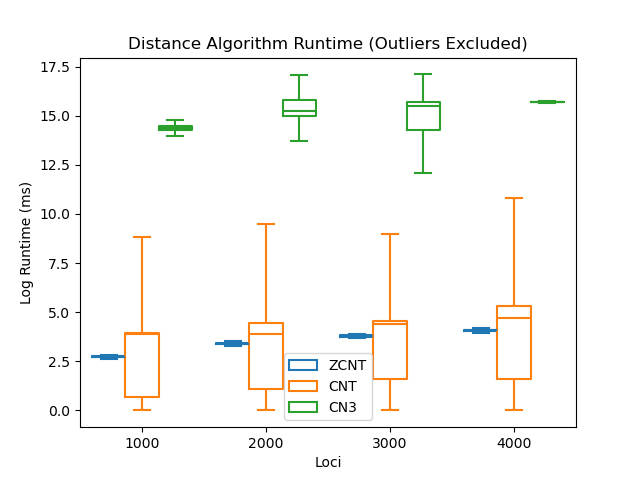
\includegraphics[width=0.45\textwidth]{figures/time_fig.png}
    \caption{This shows the running times of running the different distance methods on different numbers of loci on a logarithmic scale. All trials used 200 cells. This was computed using simulated data. The number of loci was in \{1000, 2000, 3000, 4000\}.}\label{fig:time_fig}
\end{figure} 

The results for the methods described in Section~\ref{section:comp_dist} to compare the three distance algorithms ZCNT, CNT, and CN3 are shown in Figures~\ref{fig:dist_figure_histogram} and~\ref{fig:dist_fig_box} include five suites with a constant number of 200 cells and varying numbers of loci. Most other analyses also compare across varying numbers of cells and random seeds. This analysis does not do so due to the running time involved in calculating CN3 distances. A figure demonstrating this running time is included as Figure~\ref{fig:time_fig}. This significantly higher runtime was expected due to CN3 being an $O(nB^7)$ algorithm while ZCNT and CNT are both linear time $O(n)$ algorithms. 

Figures~\ref{fig:dist_figure_histogram} and~\ref{fig:dist_fig_box} show that ZCNT and CN3 have more in common than any other pairing. However, the relative error for the grand majority of the comparison classes falls below $10\%$. Interestingly, even the most different pairing (ZCNT and CNT) mostly had errors falling below $20\%$. 

\begin{figure}[ht]
    \centering
    \includegraphics[width=0.45\textwidth]{figures/classes_hist.png}
    \caption{Absolute value of pairwise distances generated with ZCNT according to Section~\ref{section:behavior}. Class 1 is composed of ZCNT distances $\zcnt(u, v)$ where $\cnt(u, v) \neq \infty$ and $\cnt(v, u) \neq \infty$. Class 2 is composed of ZCNT distances $\zcnt(u, v)$ where exactly one of $\cnt(u, v)$ and $\cnt(v, u)$ equals $\infty$. Class 3 is composed of ZCNT distances where $\cnt(u, v) = \cnt(v, u) = \infty$. The distances are from simulated data where the number of cells was in \{200 300 400 500 600 1200\} and the number of loci was in \{1000, 2000, 3000, 4000\} across seven random seeds. The data was then binned and normalized so the area under each curve is 1.}\label{fig:classes_hist}
\end{figure}

\begin{figure}[ht]
    \centering
    \includegraphics[width=0.45\textwidth]{figures/classes_box.png}
    \caption{Absolute value of pairwise distances generated with ZCNT according to Section~\ref{section:behavior}. Note that outliers are removed from this plot. Class 1 is composed of ZCNT distances $\zcnt(u, v)$ where $\cnt(u, v) \neq \infty$ and $\cnt(v, u) \neq \infty$. Class 2 is composed of ZCNT distances $\zcnt(u, v)$ where exactly one of $\cnt(u, v)$ and $\cnt(v, u)$ equals $\infty$. Class 3 is composed of ZCNT distances where $\cnt(u, v) = \cnt(v, u) = \infty$. The distances are from simulated data where the number of cells was in \{200 300 400 500 600 1200\} and the number of loci was in \{1000, 2000, 3000, 4000\} across seven random seeds.}\label{fig:classes_box}
\end{figure}

\subsection{Behavior of ZCNT when CNT is infinite}\label{section:behavior_res}

Figures~\ref{fig:classes_hist} and~\ref{fig:classes_box} show the results from the methodology described in Section~\ref{section:behavior}. The three classes seem to all follow fairly normal distributions. Class 1 has the lowest mean while class 3 has the highest mean. This seems to signify to that reachability in CNT corresponds to lower ZCNT values. This is good because if trees minimize distance, they will also likely favor pairings in Class 1 over all other classes and favor pairings in Class 2 over pairings in Class 3. This behavior would align with biologically feasible transitions. 

\subsection{Reachability in Simulated Data}\label{section:simulated_reachability_res}

Figures~\ref{fig:illegal_desc} and~\ref{fig:illegal_edges} show the results from the methodology described in Section~\ref{section:simulated_reachability}. These show that as the number of loci increases, biologically infeasible edges become less common. The number of cells involved in the phylogeny appears to decrease the spread of the data, but not shift it. It also shows that biologically infeasible edges are relatively rare, with 22 out of 168 trees (13.09\%) having no illegal edges or ancestor-descendant relationships. The rate of illegal edges is very infrequent with is very small. Even the tree with the most illegal edges has at most 7.36\% of illegal edges. 

\begin{figure}[ht]
    \centering
    \includegraphics[width=0.45\textwidth]{figures/illegal_desc.png} 
    \caption{The percentage of overall ancestor-descendant pairs in Lazac-produced trees on simulated data where it would be biologically infeasible for the descendant to be produced from the ancestor. The number of cells was in \{200 300 400 500 600 1200\} and the number of loci was in \{1000, 2000, 3000, 4000\} across seven random seeds.}\label{fig:illegal_desc}
\end{figure}

\begin{figure}[ht]
    \centering
    \includegraphics[width=0.45\textwidth]{figures/illegal_edges.png}
    \caption{The percentage of overall edges in Lazac-produced trees on simulated data where it would be biologically infeasible for the child to be produced from the parent. The number of cells was in \{200 300 400 500 600 1200\} and the number of loci was in \{1000, 2000, 3000, 4000\} across seven random seeds.}\label{fig:illegal_edges}
\end{figure}

\begin{figure}[ht]
    \centering
    \includegraphics[width=0.45\textwidth]{figures/cumulative_plot.png}
    \caption{This shows a cumulative plot that shows what percentage of simulated trees contain biologically infeasible edges or ancestor-descendent relationships. The number of cells was in \{200 300 400 500 600 1200\} and the number of loci was in \{1000, 2000, 3000, 4000\} across seven random seeds.}\label{fig:cumulative_trees}
\end{figure}

Figure~\ref{fig:cumulative_trees} shows the cumulative rate of illegal edges or ancestor-descendant relationships. Illegal edges are the source of illegal ancestor-descendant relationships so the ancestor-descendant curve is just a horizontally stretched version of the illegal edges curve. The amount of stretch shows how many cells are descended from illegal edges. 

The plot shows that more than half the trees have fewer than 2.5\% illegal edges. The trees with the fewest illegal edges don't appear to have many descendants of those illegal relationships as shown by the curves matching for the first portion of the graph. This implies that for those trees, the ZCNT model predicts decently biologically feasible trees. However, for roughly 40\% of the trees, an increasing proportion of nodes are descended from impossible transitions like zero-amplifications. 

\subsection{Reachability in Real Data}\label{section:real_reachability_res}

\begin{figure}[ht]
    \centering 
    \includegraphics[width=0.45\textwidth]{figures/classes_real_bar.png}
    \caption{The frequency distribution of classes described in Section~\ref{section:behavior} using real data. The real data is from patient 8 of the study on metastatic prostate cancer~\cite{real_data}. The data was measured across 10 cells, a maximum of 22 chromosomes per cell, and a maximum of 38 loci per chromosome. Pairwise CNT distances were generated for each cell. Then each pairing was classified as follows. Class 1 is composed of pairings where $\cnt(u, v) \neq \infty$ and $\cnt(v, u) \neq \infty$. Class 2 is composed of pairings where exactly one of $\cnt(u, v)$ and $\cnt(v, u)$ equals $\infty$. Class 3 is composed of pairings where $\cnt(u, v) = \cnt(v, u) = \infty$.}\label{fig:classes_real_bar}
\end{figure}

\begin{figure}[ht]
    \centering 
    \includegraphics[width=0.45\textwidth]{figures/classes_sim_bar.png}
    \caption{The frequency distribution of classes described in Section~\ref{section:behavior} using simulated data. The simulated data was generated such that the number of cells was in \{200 300 400 500 600 1200\} and the number of loci was in \{1000, 2000, 3000, 4000\} across seven random seeds. Pairwise CNT distances were generated for each suite and then classified as follows. Class 1 is composed of pairings where $\cnt(u, v) \neq \infty$ and $\cnt(v, u) \neq \infty$. Class 2 is composed of pairings where exactly one of $\cnt(u, v)$ and $\cnt(v, u)$ equals $\infty$. Class 3 is composed of pairings where $\cnt(u, v) = \cnt(v, u) = \infty$.}\label{fig:classes_sim_bar}
\end{figure}

Figures~\ref{fig:classes_real_bar} and~\ref{fig:classes_sim_bar} show the results from the methods described in Section~\ref{section:real_reachability}. They show that the number of pairings falling into Classes 1 and 3 are about equal in real data but the simulated data shows a preference for Class 1. 

For both kinds of data, the frequency of pairings falling into Class 2 is the highest but the peak is stronger in the real data. This could be due to several factors including the fact that there is significantly less data available for the real data compared to the simulated data. 

\subsection{ZCNT Against Symmetric CNT Distances}\label{section:symmetric_cnt_vs_zcnt_res}

\begin{figure}[ht]
    \centering 
    \includegraphics[width=0.45\textwidth]{figures/sym_fig_hist.png}
    \caption{The relative error of ZCNT against CNT measures that correct for symmetry (Median Distance and Mean Correction) on simulated data as described in Section~\ref{section:symmetric_cnt_vs_zcnt}. The distances are from simulated data where the number of cells was in {200 300 400 500 600 1200} and the number of loci was in {1000, 2000, 3000, 4000} across seven random seeds. Pairwise ZCNT and CNT distances were generated for all cells in the data. Then Mean Correction and Median Distance were calculated for all CNT distances. Pairings where the relative distance would be $\infty$ due to Mean Correction or Median Distance being $\infty$ were excluded.}\label{fig:symmetric_rel_err_hist}
\end{figure}

\begin{figure}[ht]
    \centering
    \includegraphics[width=0.45\textwidth]{figures/sym_fig_boxplot.png}
    \caption{The relative error of ZCNT against CNT measures that correct for symmetry (Median Distance and Mean Correction) on simulated data as described in Section~\ref{section:symmetric_cnt_vs_zcnt}. Note that outliers are excluded from the graph. The distances are from simulated data where the number of cells was in {200 300 400 500 600 1200} and the number of loci was in {1000, 2000, 3000, 4000} across seven random seeds. Pairwise ZCNT and CNT distances were generated for all cells in the data. Then Mean Correction and Median Distance were calculated for all CNT distances. Pairings where the relative distance would be $\infty$ due to Mean Correction or Median Distance being $\infty$ were excluded.}\label{fig:symmetric_rel_err_box}
\end{figure}

\begin{figure}[ht]
    \centering 
    \begin{tabular}{|c|c|c|c|} \hline
        Loci & Mean Correction & Median Distance & Total \\ \hline \hline
        1000 & 76.57\% & 27.67\% & 52.12\% \\ 
        2000 & 76.06\% & 29.34\% & 52.70\% \\ 
        3000 & 51.22\% & 8.91\% & 30.07\% \\ 
        4000 & 44.51\% & 5.88\% & 25.19\% \\ \hline
        Total & 62.09\% & 17.95\% & 40.02\% \\ \hline
    \end{tabular}
    \caption{The percentage of pairwise distances excluded from plots in Figures~\ref{fig:symmetric_rel_err_hist} and~\ref{fig:symmetric_rel_err_box} due to the value being $\infty$ rounded to the nearest hundredth of a percent.}\label{fig:excluded_table}
\end{figure}
    
Figures~\ref{fig:symmetric_rel_err_hist} and~\ref{fig:symmetric_rel_err_box} show the results of the methods described in Section~\ref{section:symmetric_cnt_vs_zcnt}. Figure~\ref{fig:symmetric_rel_err_hist} shows that ZCNT's relative error with Mean Correction and with Median Distance are nearly identical. Figure~\ref{fig:symmetric_rel_err_box} shows that the number of loci in the sample does not strongly affect the relative error between ZCNT and central CNT measurements. 

Figure~\ref{fig:excluded_table} shows what percentage of pairs were excluded for each kind of distance measurement. Since ZCNT always exists as a noninfinite value, this is a representation of how often Mean Correction and Median Distance came up with infinite values. It seems that the more loci there are, the smaller the percentage of pairings result in infinite values regardless of the approach. This is interesting because the number of loci does not affect relative error. This means that the excluded values due to infinite Median Distance or Mean Correction values do not strongly affect the distribution of the distances.

The percentage of pairings resulting in infinite values is substantially higher for Mean Correction than it is for Median Distance. This is to be expected because for any distance from profile $u$ to $v$, both $\cnt(u, v)$ and $\cnt(v, u)$ must be noninfinite for the Mean Correction to be noninfinite. Meanwhile for Median Distance, only one of them must be noninfinite for the resulting value to be noninfinite.